\subsection{Current Sources}\label{sec:currentsources}
The final stage of the power DAC are the current sources. They provide a differential output over a 50$\Omega$ resistor. This setup is shown in Fig. \ref{figure:Current_sources}.
\begin{figure}[h!]
\begin{center}
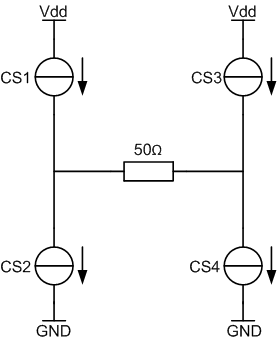
\includegraphics[width=0.4\linewidth]{Current_sources.png}
\caption{The final stage of the power DAC: The current sources which will provide the differential output through the resistor.}
\label{figure:Current_sources}
\end{center}
\end{figure}
Due to the local oscillator, the current will alternate between the path through CS1 and CS4 (see Fig.~\ref{fig:CS1CS4}) and the the path through C3 and C2. (see Fig.~\ref{fig:CS3CS2}). 
\begin{figure}
\centering
\begin{subfigure}{0.5\textwidth}
\centering
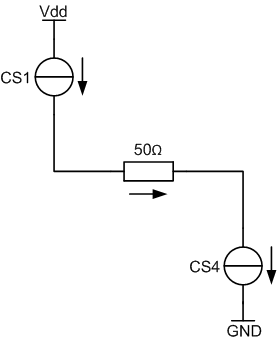
\includegraphics[width=0.4\linewidth]{Current_sources_1.png}
\caption{One current-steered cycle.}
\label{fig:CS1CS4}
\end{subfigure}
\begin{subfigure}{0.5\textwidth}
\centering
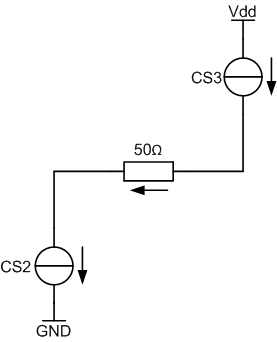
\includegraphics[width=0.4\linewidth]{Current_sources_2.png}
\caption{The other current-steered cycle. Vdd is 5V and the maximum current is 50mA.}
\label{fig:CS3CS2}
\end{subfigure}
\end{figure}
The first design parameters are the voltage supply and the switching devices. Because the DAC should be able to produce 50mA through a 50$\Omega$ resistor, the maximum voltage drop will be 2.5V. This already cancels out lower voltage supplies such as 1.2V and 2.5V. The resulting options are 3.3V and 5V. Because the stage consist of two current sources, the voltage headroom will be very limited in the 3.3V voltage supply. Therefore a 5V supply will be used as $V_{dd}$. This, along with the high switching speeds, limits the switching devices to the thick-oxide CMOS technology.\\
Due to the thick-oxide CMOS technology, the width and length of the CMOS are the only parameters. The most straightforward design method subscribes that the CMOS should always be in saturation so that the current through the CMOS is nearly independent, without channel-length modulation taken into account, of the drain-source voltage of the CMOS. This is directly related to the output impedance of the the switched current source. Therefore Eq.~\ref{eq:Overdrive} should be valid whatever the drain-source voltage.\\

\begin{equation}\label{eq:Overdrive}{V_{DS} > V_{TH} + V_{GS}}\end{equation}

The drain-source voltage of both the NMOS is minimal when the current through the resistor is maximal. This results in a minimum drain-source voltage of 1.25V. Because Eq.~\ref{eq:Overdrive} should be valid independent of the output, the maximum gate-source provided by the level shifter should be 1.95V, because the threshold voltage of the thick-oxide CMOS is 0.7V. Along with Eq.~\ref{eq:Drain current}, this would provide a viable current sink.
\begin{equation}{I_D = \frac{1}{2}\mu_n C_{ox}\frac{W}{L}(V_{GS}-V_{TH})^2(1+\lambda V_{DS})}\label{eq:Drain current}\end{equation}
So by designing a current sink which operates at a $V_{gs}$ of 1.95V, the  switching current sink wil always be in saturation. This provides a high output impedance and thus a high IMD3. Another advantage is the increase in efficiency.
Due to the difference in mobility of electrons and holes, the mobility of a electron is three times higher than the mobility of a hole, the length of the NMOS transistor will be three times higher then the length of the PMOS transistor. Though an larger length has some advantages, decrease in mismatch en less noise, it also means a larger width to maintain the required current through the transistor. A larger width however, means increasing inputcapacitance. To decrease the needed specifications on the level shifter, the length of the PMOS has been chosen to be the minimum possible with the thick-oxide technology, i.e. 300nm. The length of the NMOS is then 900nm.\\
The width of the NMOS transistors has been determined by a parametric sweep. The width can then be determined so that the current through the transistor is 3.3mA. With the circuit found in Fig. ~\ref{fig:NMOS_Width_Sweep} the result is found in Fig. ~\ref{fig:NMOS_Width_Sweep_Result}.
\begin{figure}
\begin{center}
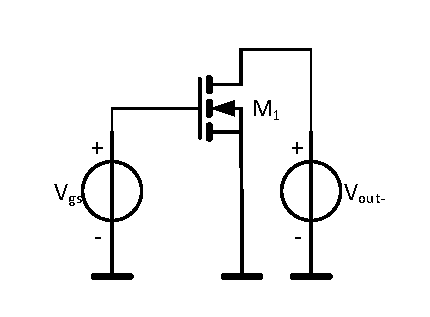
\includegraphics[width=0.4\textwidth]{NMOS_END_STAGE.pdf}
\caption{The circuit used to determine the required width of the transistor to sink 3.3mA. Vout- is 2.4167V ans Vgs is 1.95V.}
\label{fig:NMOS_Width_Sweep}
\end{center}
\end{figure}

\begin{figure}
\begin{center}
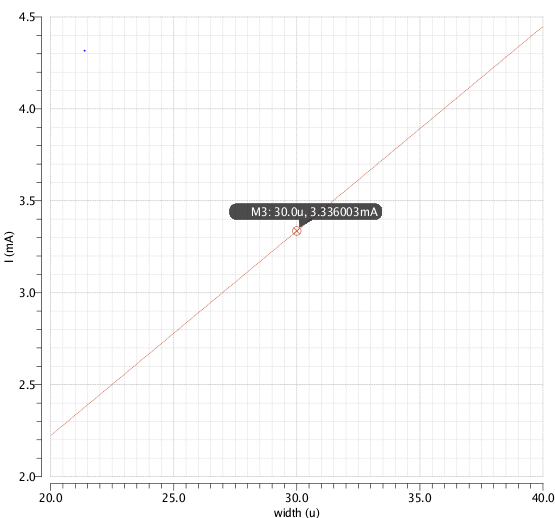
\includegraphics[width=0.4\textwidth]{NMOS_M1.png}
\caption{The current through the transistor versus its width. To make sure that the current through the transistor is 3.3mA, the width should be 30um.}
\label{fig:NMOS_Width_Sweep_Result}
\end{center}
\end{figure}

So the width of the first NMOS should be 30um to guarantee that it will sink 3.3mA when the $V_{GS}$ is 1.95V. Due to the channel-length modulation, it is not sufficient to copy the transistor 15 times. So to determine the width of the second transistor, another transistor will be added to the circuit in Fig. ~\ref{fig:NMOS_Width_Sweep} and the $V_{out-}$ will be altered to 2.333V. Then the sweep will take place again until the width has been found for which the circuit sinks 6.667mA. This will be repeated until 15 transistor are switched in parallel and are able to sink 50mA. The list of all widths can be found in table ~\ref{Tab:NMOS} in the appendix.\\
The same technique has been used for the PMOS transistors. Due to the dummy technology, which was not able to simulate width over 100um, each bit will be represented by to PMOS in parallel so that the width is maintained within the 100um. This list can also be found in the appendix, table ~\ref{Tab:PMOS}.\\

When all of these transistors are designed in a single set-up, that is a setup as seen in ~\ref{fig:CS1CS4}, a sweep can be made through all bits. The results can be found in Fig. ~\ref{fig:Final_result}.
\begin{figure}[ht!]
\begin{center}
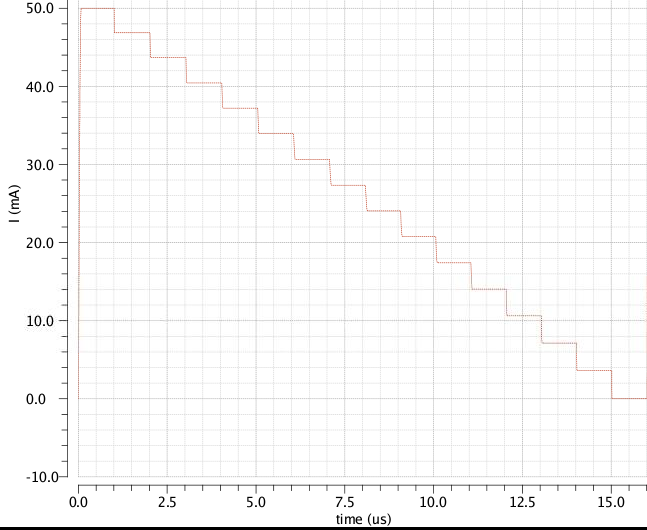
\includegraphics[width=0.4\textwidth]{Current_Cycle_Endstage.png}
\caption{A sweep through all possible currents, with a maximum of 50mA and a minimum of 0mA.}
\label{fig:Final_result}
\end{center}
\end{figure}

Next paper I will elaborate on the results with the chosen transistors. 